\section{Mediciones}

\subsection{Se realizaron comparaciones entre backtracking y programación lineal}

\begin{figure}[H]
    \centering
    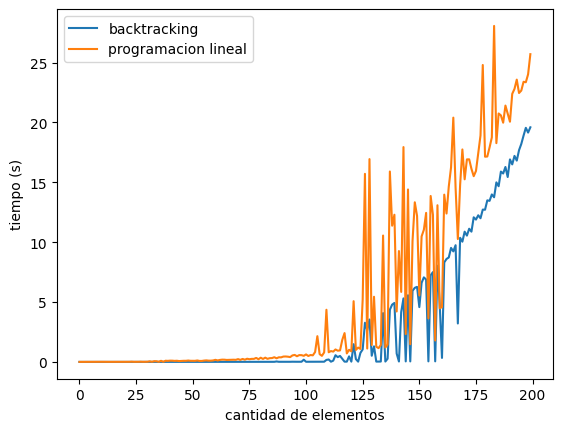
\includegraphics[width=1\textwidth]{img/backvslp.png}
\end{figure}

Backtracking obtiene mejores tiempo de ejecución que programación lineal para encontrar la solución óptima.

\subsection{Se realizaron comparaciones entre greedy y programación lineal relajada}

\begin{figure}[H]
    \centering
    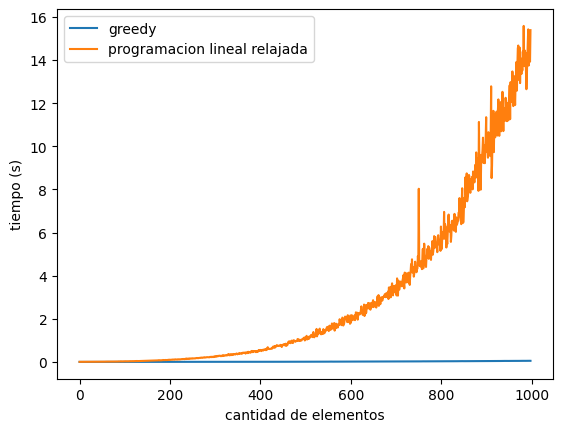
\includegraphics[width=1\textwidth]{img/greedyvslprx.png}
\end{figure}

Greedy demora mucho menos tiempo que programación lineal relajada para encontrar una aproximación, pero la aproximación otorgada es peor.